\section{Validation}
\label{sec:validation}

Our objective is to validate the self-adaptive middleware Tekio built using an OSGi component framework (Eclipse Equinox Cited). The validation aims to encourage the reuse of legacy components in modern self-adaptive frameworks. Our case study is a self-adaptive computer vision system built using Tekio. We choose the representative computer vision domain for a number of reasons: (a) they process large amounts of input data with variations in resolution and content of images, (b) they often require high-throughput and low latency and can run on various operating platforms, (c) they solicit the use of hardware resources such as cameras, high-end  servers, and actuators, and (d) computer vision applications require complex software components involving large databases, file systems, and image processing algorithms.

We are intrigued by two principal questions that we address experimentally:
\noindent \textbf{Q1}:How much performance is compromised due to the use of self-adaptive middleware on a native implementation?
\noindent \textbf{Q2}:How often the system can adapt while maintaining a minimal QoS?

The experimental setup to answer these questions is presented in Section \ref{sec:sec:experimentalsetup}. Finally, we present results of our experiments and discuss them in Section \ref{sec:sec:resultsdiscussion}.


\subsection{Experimental Setup}
\label{sec:sec:experimentalsetup}

Dynamic adaptation is between different system configurations of video processing components handled by Tekio. A configuration is a specific set of components and its parameters. The components in the configuration are composed in a video processing chain/pipeline. In our experiments we implement a total of six configurations in Figure \ref{fig:configurations}.

\begin{figure*}[bht]
   %\fbox{
 %\vspace{-20pt}
 \centering
 \hbox{\begin{minipage}[c]{0.4\textwidth}
       Configurations\\
		\begin{tabular}{ll}
			\hline
	       Number & Name \\ \hline
	       \textbf{C1} & SMOOTH\_SEGMENTATION \\
	       \textbf{C2} & FGD\_SEGMENTATION \\
	       \textbf{C3} & PYRAMID\_SEGMENTATION \\
	       \textbf{C4} & INTRUSION\_DETECTION \\
	       \textbf{C5} & FACE\_DETECTION \\
	       \textbf{C6} & FACE\_DETECTION\_FGD \\ \hline
	       \end{tabular}
   \end{minipage}
	
   \begin{minipage}[c]{0.6\textwidth}
       \begin{center}
	   Configurations Details
       \begin{tabular}{lllllll}
		\hline
       Component & C1 & C2 & C3 & C4 & C5 & C6\\ \hline
       OpenCV AVI Reader &  1 & 1 & 1 & 1 & 1 & 1\\
       Image Smoothing &  2 & $\times$ & $\times$ & 2 & $\times$ & $\times$ \\
       FGD Background Subtraction & $\times$ & 2 & $\times$ & $\times$ & $\times$ & 2\\
       Pyramid Segmentation &  $\times$ & $\times$ & 3 & $\times$ & 2 & $\times$\\
       HAAR Detection &  $\times$ & $\times$ & $\times$ & 3 & 3 & 3\\
       Image Window &  3 & 3 & 4 & 4 & 4 & 4 \\ \hline
       \end{tabular}
       \end{center}
   \end{minipage}}
  % \vspace{-30pt}
  %}
 \caption{Experimental Configurations}
  \label{fig:configurations}
\end{figure*}

%\begin{figure}
%	[H] \centering 
%	\includegraphics[scale=0.5]{images/SystemConfigurations.jpg} \caption{System Configurations} \label{fig:SystemConfigurations} 
%\end{figure}

We present the content of these configurations in Figure \ref{fig:configurations}. For example, the configuration for motion detection contains three different components (a) image acquisition that reads a video from a file, (b) image segmentation that reduces or smoothens the edges of the images, (c) blob construction  that finds the contours of objects and translates them into detected movement. 

Another dimension of variability in our experiments is the image resolution. The input to the video processing chain is 1020 frames of video in an office space available in three different resolutions:1) High, 1024x720 pixels with a bit rate of 3,582 2) Medium, 720x400 pixels with a bit rate of 1,325 and, 3) Low, 480x272 pixels with a bit rate 681. Each experiment measures percentage of CPU usage, percentage of memory usage and FPS monitored every 5 frames. 

We evaluate the configurations based on the following metrics:
	\begin{description}
		\item[Throughput] We measure throughput using the rate at which the video processing chain processes frames per second (FPS).
		\item[Settling Time] The time the system takes to switch from the current configuration to the next. This measurement takes into account the time needed to load the new components
		\item[CPU Usage] What percentage of the processor Tekio is using at a given instant. This includes the percentage of processor used by the loaded vision components.
		\item[Memory Usage] What quantity of memory Tekio is using at any given instant. This measurement also includes includes memory used by vision components in Tekio.
	\end{description}

We design two experiments to address questions \textbf{Q1} and \textbf{Q2}:

\begin{description}	
		\item[Experiment E1] For \textbf{Q1}, we run a single configuration with three resolutions. Each system configuration is first run  with legacy static C components. Second, we run the configuration using  Tekio that handles the C components in its self-adaptive framework. The goal is to understand how much performance is lost by adding the self-adaptive layer, and whether this performance loss out costs the benefits of self-adaptation.
		
		\item[Experiment E2] For \textbf{Q2}, we run 38 pairs (without repetition) of the 6 configurations in a fixed time. First, we reconfigure 38 times in two minutes.	Secondly, we  decrease the time limit to 90 seconds and continue reducing to 60, 45, 30, 15, 10, 5, 4, 3, 2, 1 second(s). The purpose here is to figure how the system is affected by the stress to adapt quickly in fixed time. Can we determine when the system stops functioning properly due to a very high frequency of adaptation?
		
	\end{description}
	
All experiments to answer our empirical questions  are executed on an iMac with the Intel Core i3 Processor of 3.06GHz and 4GB 1333 MHz DDR3.
	
\subsection{Results and Discussion}
\label{sec:sec:resultsdiscussion}

We summarize the results of executing experiment \textbf{E1} in Figure \ref{fig:performanceComparison} and  \textbf{E2} in Figure \ref{fig:stressTesting}.
	%graphs
	\begin{figure*}
	%	[H] \centering %1415 × 415
		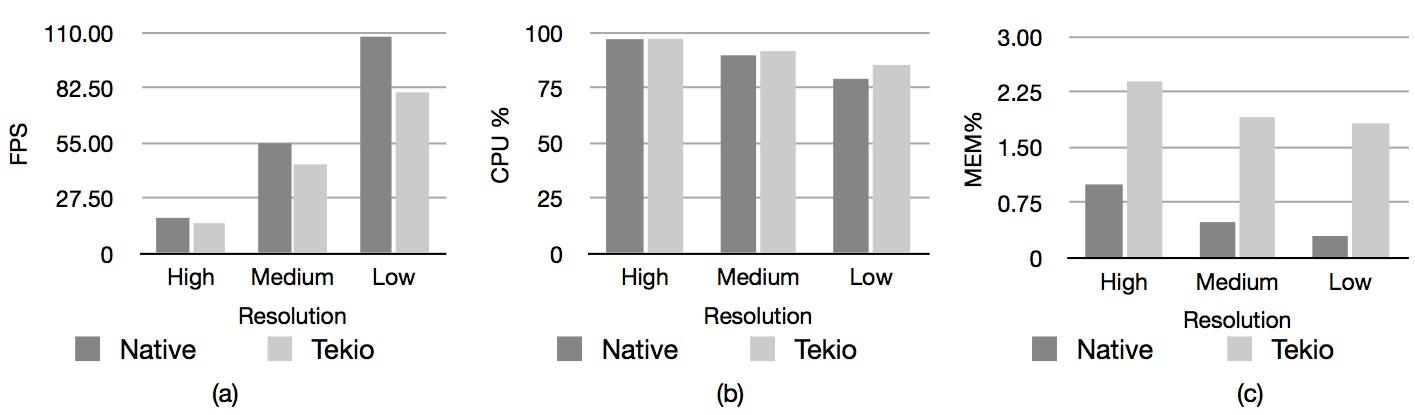
\includegraphics[scale=0.7]{images/MotionDetectionComparison.jpg} 
		\caption{Performance Comparison of Legacy and Self-adaptive for Motion Detection (a) Frame Rate (b) CPU Usage (c) Memory Usage }
		 \label{fig:performanceComparison} 
	\end{figure*}
	
	\begin{figure*}
	%	[H] \centering 
		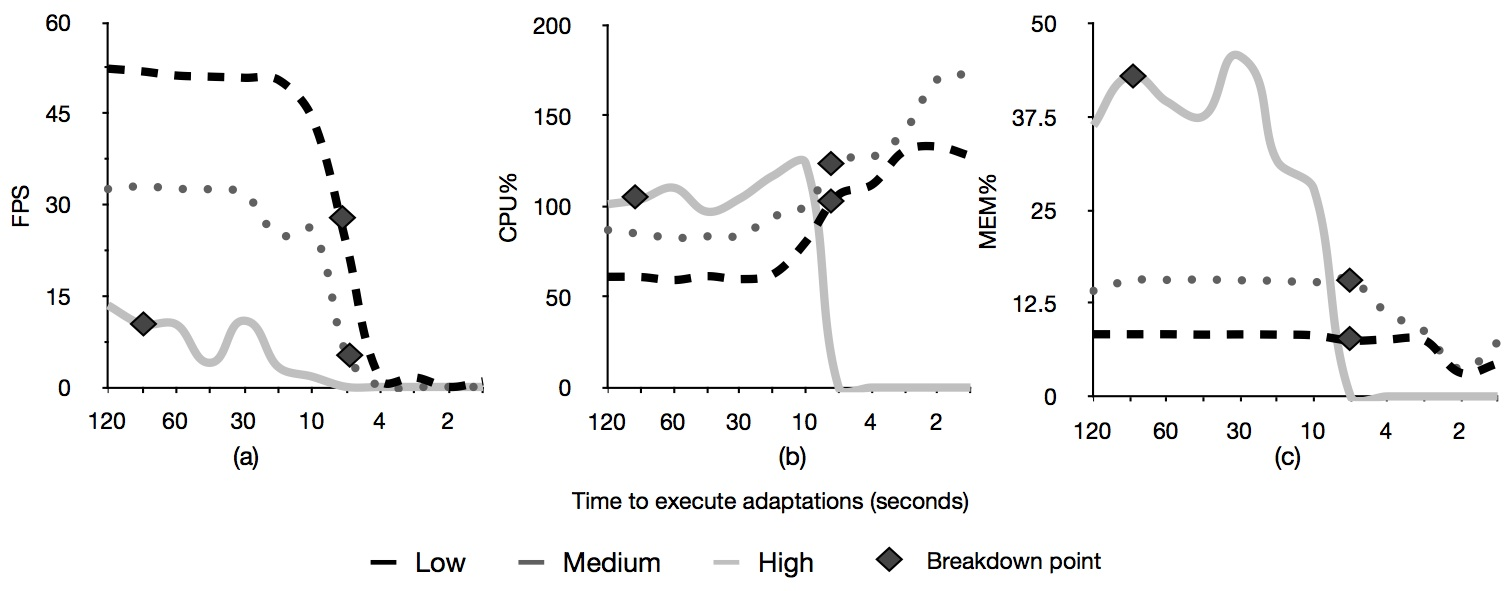
\includegraphics[scale=0.7]{images/StressTesting.jpg}
		 \caption{Stress Testing All Switches to Motion Detection (a) Frame Rate (b) CPU Usage (c) Memory Usage}
		 \label{fig:stressTesting} 
	\end{figure*}
	%How question where answer


In this section, we summarize and present the results of the experimental executions. 


We execute  \textbf{Experiment E1} to address \textbf{Question Q1}. In Figure \ref{fig:performanceComparison}, we compare a legacy  implementation of motion detection in C with motion detection within the self-adaptive framework Tekio. As expected, in Figure \ref{fig:performanceComparison} (a) we observe that the frame rate is \emph{slightly higher} for a native/legacy implementation of motion detection compared to Tekio for all three resolutions low, medium, and high. The CPU usage for both native and Tekio is similar as shown in Figure \ref{fig:performanceComparison} (b). However, we observe large difference in memory usage in Tekio compared to a native implementation as seen in Figure \ref{fig:performanceComparison} (c). The OSGi framework used to develop Tekio uses up considerable amount of memory compared to the native implementation. However, the upper limit is around 2.25\% of main memory (4Gb) which is largely acceptable. 

We execute \textbf{Experiment E2} to address \textbf{Question Q2}. We switch between pairs of configuration using Tekio. In all possible 38 pairs of configurations we choose to show 6 pairs where we switch to motion detection from any given configuration with varying time limits and resolutions. The results for low, medium, and high resolution input videos are are shown in Figure \ref{fig:stressTesting}. In  Figure \ref{fig:stressTesting} (a), we observe that frame rate starts dropping at 90 seconds time bound for high resolution while 5 seconds time bound for low and medium resolution videos. This implies that a high frequency of adaptation is not suitable for high resolution images while we may expect to adapt several times for lower resolution videos. The CPU usage drops for high resolution after its break point as seen in Figure \ref{fig:performanceComparison} (b). However, as the frequency of adaptation increases for low and medium the CPU usage increases beyond using a single CPU (upto 170\%). Finally,  in Figure \ref{fig:performanceComparison} (c), we notice that memory usage for high resolution is initially very high but gradually drops after the break point. The memory usage remains relatively static for low and medium resolution but drops after the break point. 

We define the time required for the system to settle down into a state which produces meaningful results as settling time. In conclusion, we observe that most of the \emph{settling times} are very low. However,  if the system adapts very fast (about 0.25 milliseconds per adaptation) the system can begin to fail depending on the load and video resolution. However, most importantly Tekio does not crash, it simply does not produce results and continues running, this is possible because the algorithms do not produce any exceptions. In future work, we would like to see if Tekio can recover from bursts of high loads automatically without crashing.
